
\chapter*{Benchmarks and error framework}
\label{sec:org46e470c}

\section*{Benchmarks}
\label{sec:org570cc00}

As stated in the Introduction, the research was conducted in order to analyze the different metrics to assert the quality of a mapping algorithm.
Consequently, we used a classic technique, the benchmarking technique.
In general computing, a benchmark is a program or a set of programs used to assess the performance of the host technology.
In our case, a benchmark would be a quantum algorithm that we will map to the SC chips constraints and then simulate aiming to use them to understand the different metrics.
Under this approach, it was decided that the best methodology would go through four different steps.
First, we built a list of quantum algorithms as benchmarks.
We opted to collect a big variety of different algorithms from different sources and libraries with a view to classify them and select the most interesting ones afterwards.
As it is common to find in the literature [REFER ALL THE PAPERS WITH LIST OF REAL BENCHMARKS], we also decided the benchmarks to be real and useful quantum algorithms, instead of random circuits.

from RevLib \cite{Wille_2008}, ScaffCC \cite{JavadiAbhari_2015}, Zulehner's paper \cite{zulehner17:effic_method_mappin_quant_circuit} and QLib \cite{Lin_2014}.


Then I had to translate them from its QASM version to OpenQL.

And finally compile them.


Steps:

\begin{enumerate}
\item Build algorithms list       
\begin{enumerate}
\item Gather the algorithms from \cite{zulehner17:effic_method_mappin_quant_circuit} and \cite{Lin_2014}.
\item Translate them from its QASM version to OpenQL.
\item Compile OpenQL files to QASM.
\end{enumerate}
\item Algorithms profile (source, number of qubits, number of gates, gates percentage, \ldots{}).
\item Algorithms classification.
\item Check algorithm correctness.
\begin{enumerate}
\item Are the original algorithms correct? \(\to\) Check behaviour in the IBM Simulator.
\item Is my translation correct? \(\to\) Simulate them in QX and compare the results with the ones of the previous step.
\item Are the algorithms working as expected? \(\to\) check if the results are the ones that the algorithm should have.
\end{enumerate}
\end{enumerate}

\begin{figure}
\centering
\resizebox{0.75\textwidth}{!}{
\begin{tikzpicture}[>=stealth',shorten >=1pt,auto,node distance=0.7cm, thick,main node/.style={}]
    \fill[orange!40] (2,2) circle (.08cm) coordinate (Z);
    \fill[cyan!30] (3,6) circle (1.6cm) coordinate (R);
    \fill[purple!50] (7,5) circle (.1cm) coordinate (S);
    \fill[teal!40] (8,2) circle (1cm) coordinate (Q);
    \draw[gray,dashed] (5,4) ellipse (6cm and 4cm) coordinate (A);
    \draw (4,0) -- coordinate (L) (10,6.4) coordinate (Le);
 %\node[main node] (1) [left of R] {RevLib};
\node[main node] at (3,6) {RevLib};
\node[main node] (2) [above of=Z] {Others from Zulehner's paper};
\node[main node] (3) [above of=S] {ScaffCC};
%\node[main node] (4) [above right of Q] {QLib};
\node[main node] at (8,2) {QLib};
\node[main node,draw] (5) [above left  of=L] {OPENQASM};
\node[main node,draw] (6) [below of=Le] {QLib QASM};
\end{tikzpicture}
}
\label{fig:benchmarks_graph}
\caption{Graph depicting the amount of benchmarks per source. The line splits the source depending on the description programming language}
\end{figure}

\begin{itemize}
\item :B\(_{\text{onlyenv}}\):
\label{sec:orgf0004af}
\begin{itemize}
\item OPENQASM
\begin{itemize}
\item RevLib (55)
\item ScaffCC (3)
\item Others from Zulehner's paper (1)
\end{itemize}
\item QLib QASM
\begin{itemize}
\item QLib (7)
\end{itemize}
\end{itemize}


\item :B\(_{\text{onlyenv}}\):
\label{sec:org952053b}
\begin{itemize}
\item OPENQASM
\begin{itemize}
\item RevLib (52)
\item \sout{ScaffCC}
\item Others from Zulehner's paper (1)
\end{itemize}
\item QLib QASM
\begin{itemize}
\item QLib (3)
\end{itemize}
\end{itemize}
\item Benchmarks data analysis
\label{sec:orgf489be9}

\item :B\(_{\text{onlyenv}}\):
\label{sec:org231da8d}
The Clifford+T quantum algorithms gathered are not in pure QASM:

\item :B\(_{\text{onlyenv}}\):
\label{sec:org0d768a2}
After the translation, despite gates that OpenQL is not able to decompose yet, the compiled QASM files are:



\item OpenQL Translation
\label{sec:orgb1d53c0}
So they should be translated to OpenQL an then compiled to QASM.

\item {\bfseries\sffamily TODO} :B\(_{\text{noteNH}}\):
\label{sec:org5fc32c8}
Now, I'm going to show you how the benchmarks are.

Most of them are written in OPENQASM and are from RevLib.

Moreover, Leon has contributed uploading more, but I haven't merge those with the ones I am describing.

\hline

Some of them have arbitrary rotation gates, which decomposition is not included yet in OpenQL, so I'm not going to translate them for now.


\item Benchmarks Classification
\label{sec:orgcb72ff5}
\end{itemize}

\subsection*{Benchmarks formation and classification}
\label{sec:orge03a2e5}


\begin{itemize}
\item Benchmarks statistics
\label{sec:orgc7ef40d}

\begin{itemize}
\item Statistics
\label{sec:org7031de1}

\begin{itemize}
\item Number of different algorithms (without the decomposition): 53+3 = 56
\item The highest amount of gates: \texttt{hwb9\_119} with 207775 gates
\end{itemize}


\item :BMCOL:
\label{sec:org0b5d5d5}
You can find much more information in the \href{https://github.com/QE-Lab/qbench}{qbench} repository in GitHub or in my thesis notes in ShareLaTeX.


\item {\bfseries\sffamily TODO} :B\(_{\text{noteNH}}\):
\label{sec:org6ba5b8f}
After the translation, we have 56 different algorithms, in which the higgest amount of gates is around 208 000 gates.

Also I'm going to show you how is the qbench repo right now.


Things that may interest them:

\begin{itemize}
\item See the OpenQL code and the QASM code
\item The organization of the repository
\item The Benchmarks profile
\item The configuration file of the compilation
\end{itemize}

\item {\bfseries\sffamily TODO} :B\(_{\text{noteNH}}\):
\label{sec:org5556120}
After the building step, as I've already shown you, the profile realization and classification steps came.

Finally, right now I'm checking the algorithm correctness.
\end{itemize}
\end{itemize}

\section*{Error framework}
\label{sec:orgfdd9514}
In this section we introduce the framework we developed in order to analyze the quantum metrics.

\subsection*{Compiler (OpenQL, cQASM)?}
\label{sec:org229ed29}

[Intro]


\begin{figure}[htbp]
\centering
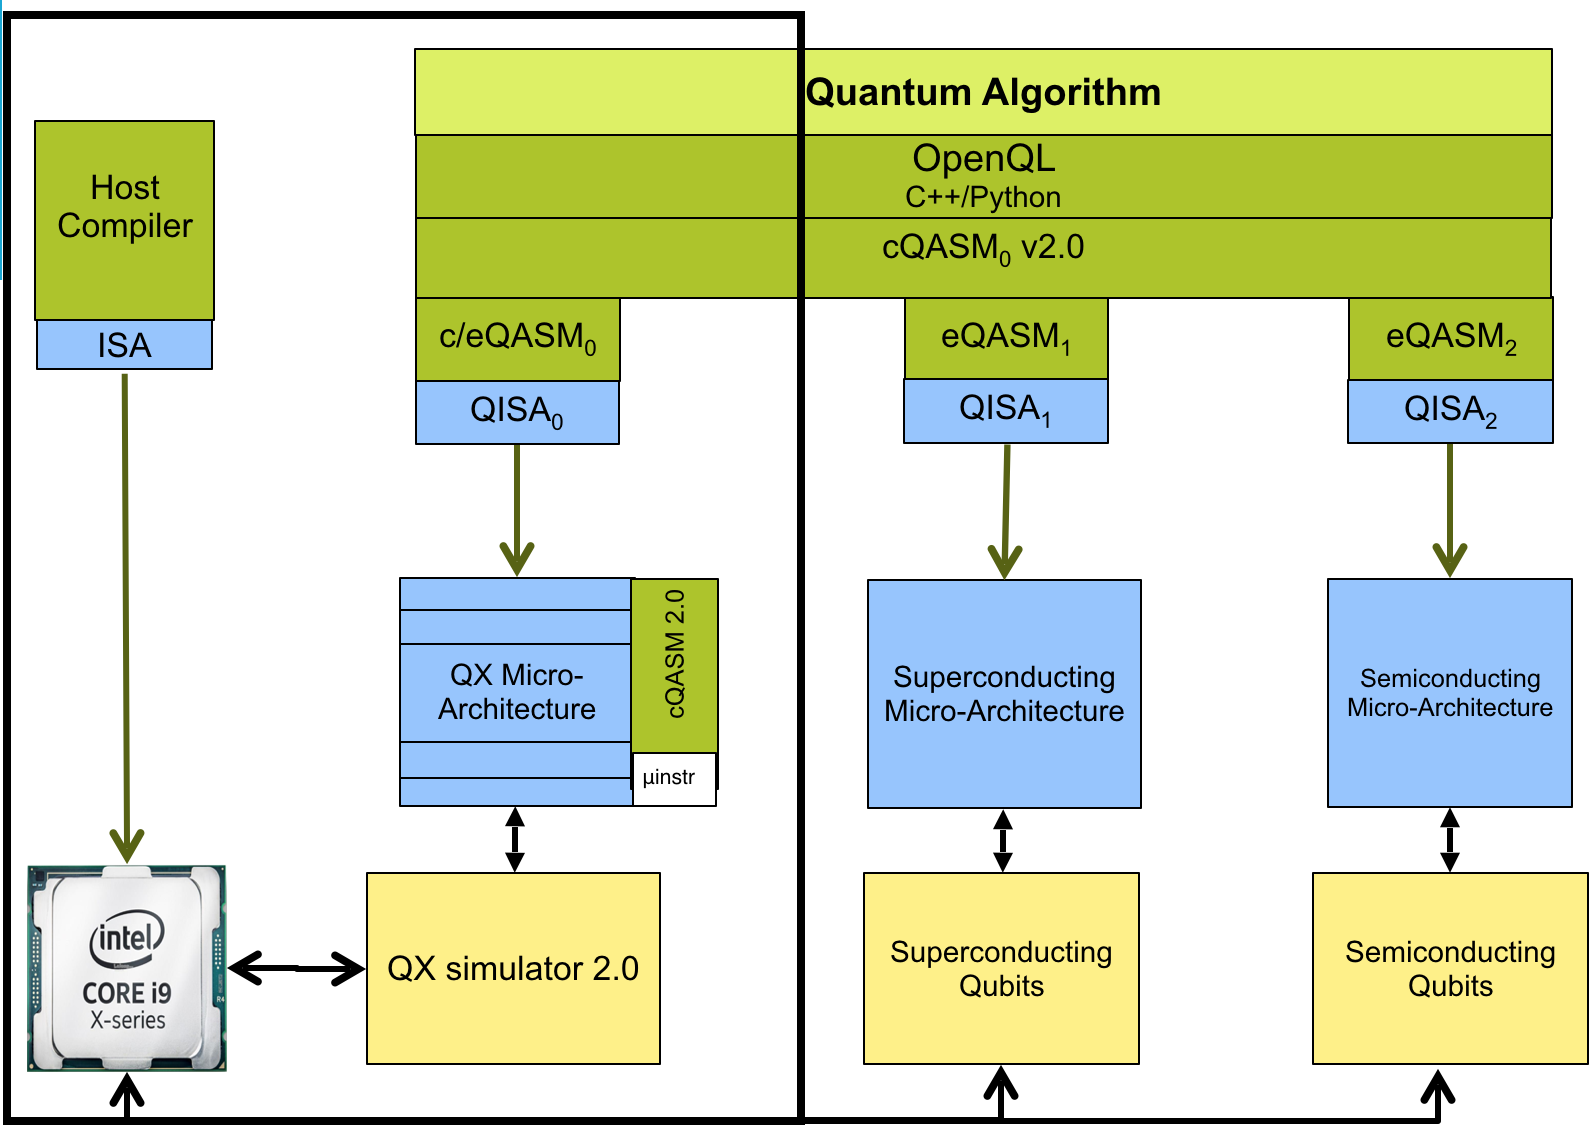
\includegraphics[width=\textwidth]{figures/layers.png}
\caption{\label{fig:orgc6550a9}
Compilation layers}
\end{figure}


\begin{itemize}
\item cQASM
\label{sec:org7b86bba}


\item OpenQL
\label{sec:orgbc715e2}

\begin{figure}[htbp]
\centering
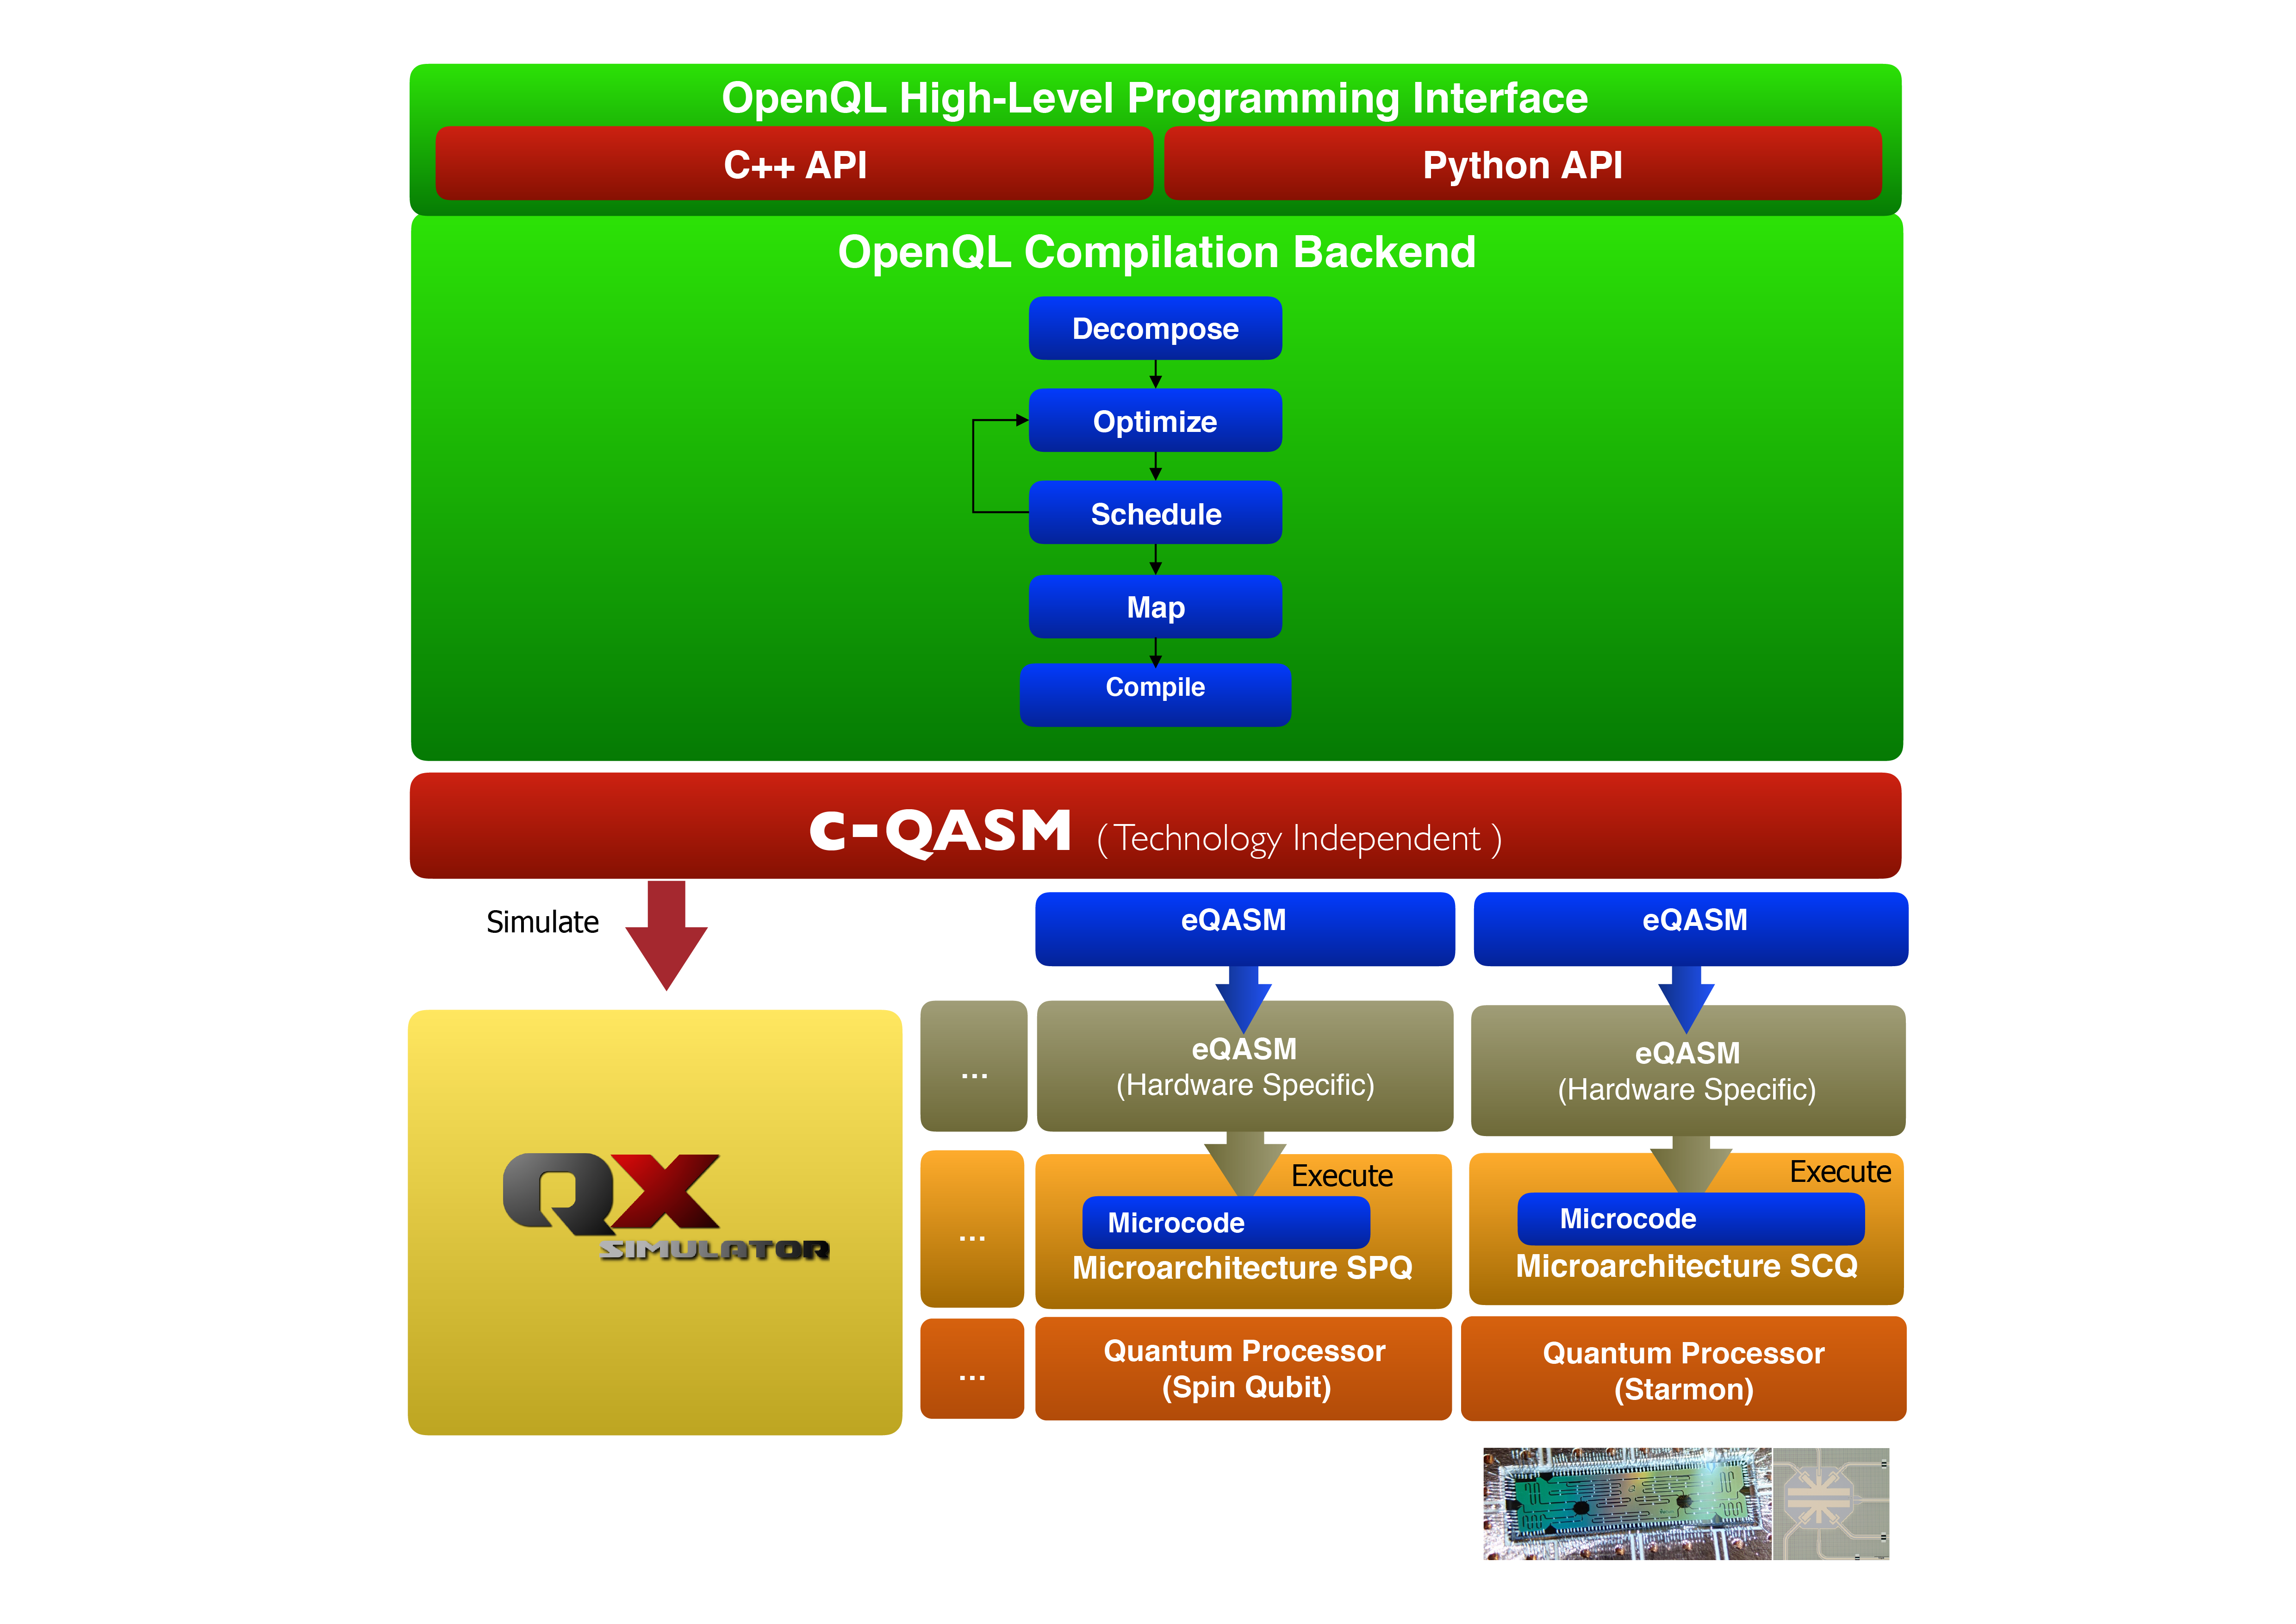
\includegraphics[width=0.9\textwidth]{figures/openql.png}
\caption{\label{fig:org3add541}
OpenQL diagram}
\end{figure}

\begin{figure}
\centering
\begin{minipage}{\textwidth}

\begin{minted}[frame=lines,fontsize=\scriptsize,linenos,breaklines,breakanywhere]{python}

from openql import openql as ql
import os
import argparse

def circuit(config_file, scheduler='ASAP', uniform_sched= 'no', mapper='base', initial_placement='no', output_dir_name='test_output', optimize='no', measurement=True, log_level='LOG_WARNING'):
    curdir = os.path.dirname(__file__)
    output_dir = os.path.join(curdir, output_dir_name)
    ql.set_option('output_dir', output_dir)
    ql.set_option('optimize', optimize)
    ql.set_option('scheduler', scheduler)
    ql.set_option('scheduler_uniform', uniform_sched)
    ql.set_option('mapper', mapper)
    ql.set_option('initialplace', initial_placement)
    ql.set_option('log_level', log_level)

    config_fn = os.path.join(curdir, config_file)

    platform  = ql.Platform('starmon', config_fn)
    sweep_points = [1,2]
    num_circuits = 1
    num_qubits = 6
    p = ql.Program('graycode6', platform, num_qubits)
    p.set_sweep_points(sweep_points, num_circuits)
    k = ql.Kernel('graycode6', platform, num_qubits)
    k.gate('cnot',[1,0])
    k.gate('cnot',[2,1])
    k.gate('cnot',[3,2])
    k.gate('cnot',[4,3])
    k.gate('cnot',[5,4])

    if measurement:
	for q in range(num_qubits):
	    k.gate('measure', [q])

    p.add_kernel(k)
    p.compile()

\end{minted}

\caption{QASM code describing the Gray code algorithm.}
\label{code:qasm_gray_code}
\end{minipage}
\end{figure}
\end{itemize}

\subsection*{{\bfseries\sffamily TODO} quantumsim}
\label{sec:org344c0ef}

\begin{itemize}
\item Error model parameters
\label{sec:org07a24b2}

\begin{table}[htbp]
\caption{\label{tab:org4395d9d}
Main error model parameters for simulation}
\centering
\tiny
\begin{tabular}{lccp{7cm}}
\hline
Parameter & Symbol & Value & Explanation and notes\\
\hline
Qubit relaxation time & \(T_1\) & 30 \(\mu s\) & Only affects qubits in the excited state. Consistent set of values: [20 - 100 \(\mu s\)]\\
Qubit dephasing time (white noise) & \(T_{\phi}\) & 60 \(\mu s\) & Consistent set of values would be \(2 T_1\) or \(\infty\) (all white noise dephasing eliminated)\\
Decay time & \(T_2\) & 30 \(\mu s\) & \(\frac{1}{T_2} = \frac{1}{T_{\phi}} + \frac{1}{2 T_1}\)\\
Single-qubit gate time & \(T_{g,1Q}\) & 20 ns & \\
Two-qubit gate time & \(T_{g,2Q}\) & 40 ns & \\
Measurement time & \(\tau_m\) & 300 ns & \\
Depletion time & \(\tau_d\) & 300 ns & ?\\
Fast Measurement time & \(\tau_m^{\text{fast}}\) & 100 ns & \\
Fast Depletion time & \(\tau_d^{\text{fast}}\) & 100 ns & ?\\
Readout infidelity & \(\epsilon_{RO}\) & 5\,(-3) & \\
Physical qubit Fidelity & \(\mathcal{F}_{phys} (t)\) & - & \(\mathcal{F}_{phys} (t) = \frac{1}{6}\left(1 + e^{-\frac{t}{T_1}}\right) + \frac{1}{3}\left(1 + e^{-t\left(\frac{1}{2 T_1} + \frac{1}{T_{\phi}}\right)} \right)\)\\
Physical qubit error rate & \(\epsilon_{phys}\) & - & \(\epsilon_{phys} = - \tau_{circuit} \frac{d \mathcal{F}_{phys} (t)}{dt} \textbar_{t=0}=\frac{\tau_{circuit}}{3 T_1}+\frac{\tau_{circuit}}{3 T_{\phi}}\)\\
In-axis rotation error & \(p_{axis}\) & 1\,(-4) & Decay corresponding to shrinking along the y axis because of the single-qubit gates depolarizing noise\\
In-plane rotation error & \(p_{plane}\) & 5\,(-4) & Decay corresponding to shrinking along the x and z axis because of the single-qubit gates depolarizing noise\\
\hline
\end{tabular}
\end{table}

\item Error models
\label{sec:org8dffb3d}

In the quantumsim module, all gates are applied in the Pauli transfer matrix representation:

$$(R_{\Lambda})_{ij} = \frac{1}{2} Tr(\sigma_i \Lambda \sigma_j)$$

where \(\sigma_i\) are the Pauli operators: \(\sigma_0 = I\), \(\sigma_1 = X\), \(\sigma_2 = Y\), \(\sigma_3 = Z\)

\begin{itemize}
\item Qubit Idling
\label{sec:org8422bbd}

While idling for a time \(t\), a transmon in \(|1\rangle\) or in superposition could relax to \(|0\rangle\) or acquire random quantum phase shifts due to \(1/f\) noise sources (flux noise) or others.
The dephasing effect only appears in a superposition state.

\begin{itemize}
\item Amplitude-phase damping model
\label{sec:org2611c22}

$$R_{\Lambda_{T_1}} = \begin{bmatrix}
 1 & 0 & 0 & 0 \\
 0 & \sqrt{1 - p_1} & 0 & 0 \\
 0 & 0 & \sqrt{1 - p_1} & 0 \\
 p_1 & 0 & 0 & 1 - p_1 \\
\end{bmatrix}$$


$$R_{\Lambda_{T_{\phi}}} = \begin{bmatrix}
 1 & 0 & 0 & 0 \\
 0 & \sqrt{1 - p_{\phi}} & 0 & 0 \\
 0 & 0 & \sqrt{1 - p_{\phi}} & 0 \\
 0 & 0 & 0 & 1 \\
\end{bmatrix}$$

with \(p_1 = 1 - e^{-\frac{t}{T_1}}\) and \(p_{\phi} = 1 - e^{-\frac{t}{T_{\phi}}}\) that are the probabilities for relaxation and pure dephasing, respectively.

\item Qubit idling
\label{sec:org5e88c8d}

Idling for a duration \(t\):

$$R_{AP (t)} = R_{\Lambda_{T_1}} R_{\Lambda_{T_{\phi}}}$$
\end{itemize}

\item Single-qubit \(R_y(\pi /2)\) rotations
\label{sec:org6ed137e}

"Single-qubit gates [\ldots{}] errors can mostly be attributed to Markovian noise. [\ldots{}] we thus model these errors as Markovian".

"Single-qubit rotations are modeled by sandwiching an instantaneous Pauli transfer matrix, representing the rotation, with periods of duration \(\frac{\tau_{g,1Q}}{2}\) of amplitude and phase damping.
This allows to model the gate for different \(T_1\) and \(T_{\phi}\) [\ldots{}]
However, [\ldots{}] actual gates are more accurately described when adding a [\ldots{}] depolarizing noise to the instantaneous part.
In the Bloch sphere, this decay corresponds to shrinking toward the origin, with factor  \(1 - p_{axis}\) along the y axis and \(1 - p_{plane}\) along the x- and z-axes":

$$R_{R_y (\pi /2)} = R_{AP (\frac{\tau_{g,1Q}}{2})} R_{R_y (\pi /2)}' R_{dep} R_{AP (\frac{\tau_{g,1Q}}{2})}$$

where

$$R_{dep} = \begin{bmatrix}
 1 & 0 & 0 & 0 \\
 0 & 1 - p_{plane} & 0 & 0 \\
 0 & 0 & 1 - p_{axis} & 0 \\
 0 & 0 & 0 & 1 - p_{plane} \\
\end{bmatrix}$$

and \(R_{R_y (\pi/2)}'\) is the Pauli transfer matrix describing the theoretical \(\pi /2\) rotation along the y axis.

\item CZ gates
\label{sec:orgb6f3ece}

"The C-Z gate is achieved by flux pulsing a transmon into the \(|11\rangle \leftrightarrow |02\rangle\) avoided crossing with another, where the 2 denotes the second-excited state of the fluxed transmon.
Holding the transmons here for \(\tau_{g,2Q}\) causes the probability amplitudes of \(|01\rangle\) and \(|11\rangle\) to acquire phases[\ldots{}]

Our full (but simplistic) model of the CZ gate consists of an instantaneous CZ gate with single-qubit phase error \(\delta_{\phi_{1Q}}\) and two-qubit phase error \(\delta_{\phi_{2Q}} = \frac{\delta_{\phi_{1Q}}}{2}\), sandwiched by idling intervals of duration \(\frac{\tau_{g,2Q}}{2}\)."


\item Measurement
\label{sec:orgdbc0cad}

\begin{figure}[htbp]
\centering
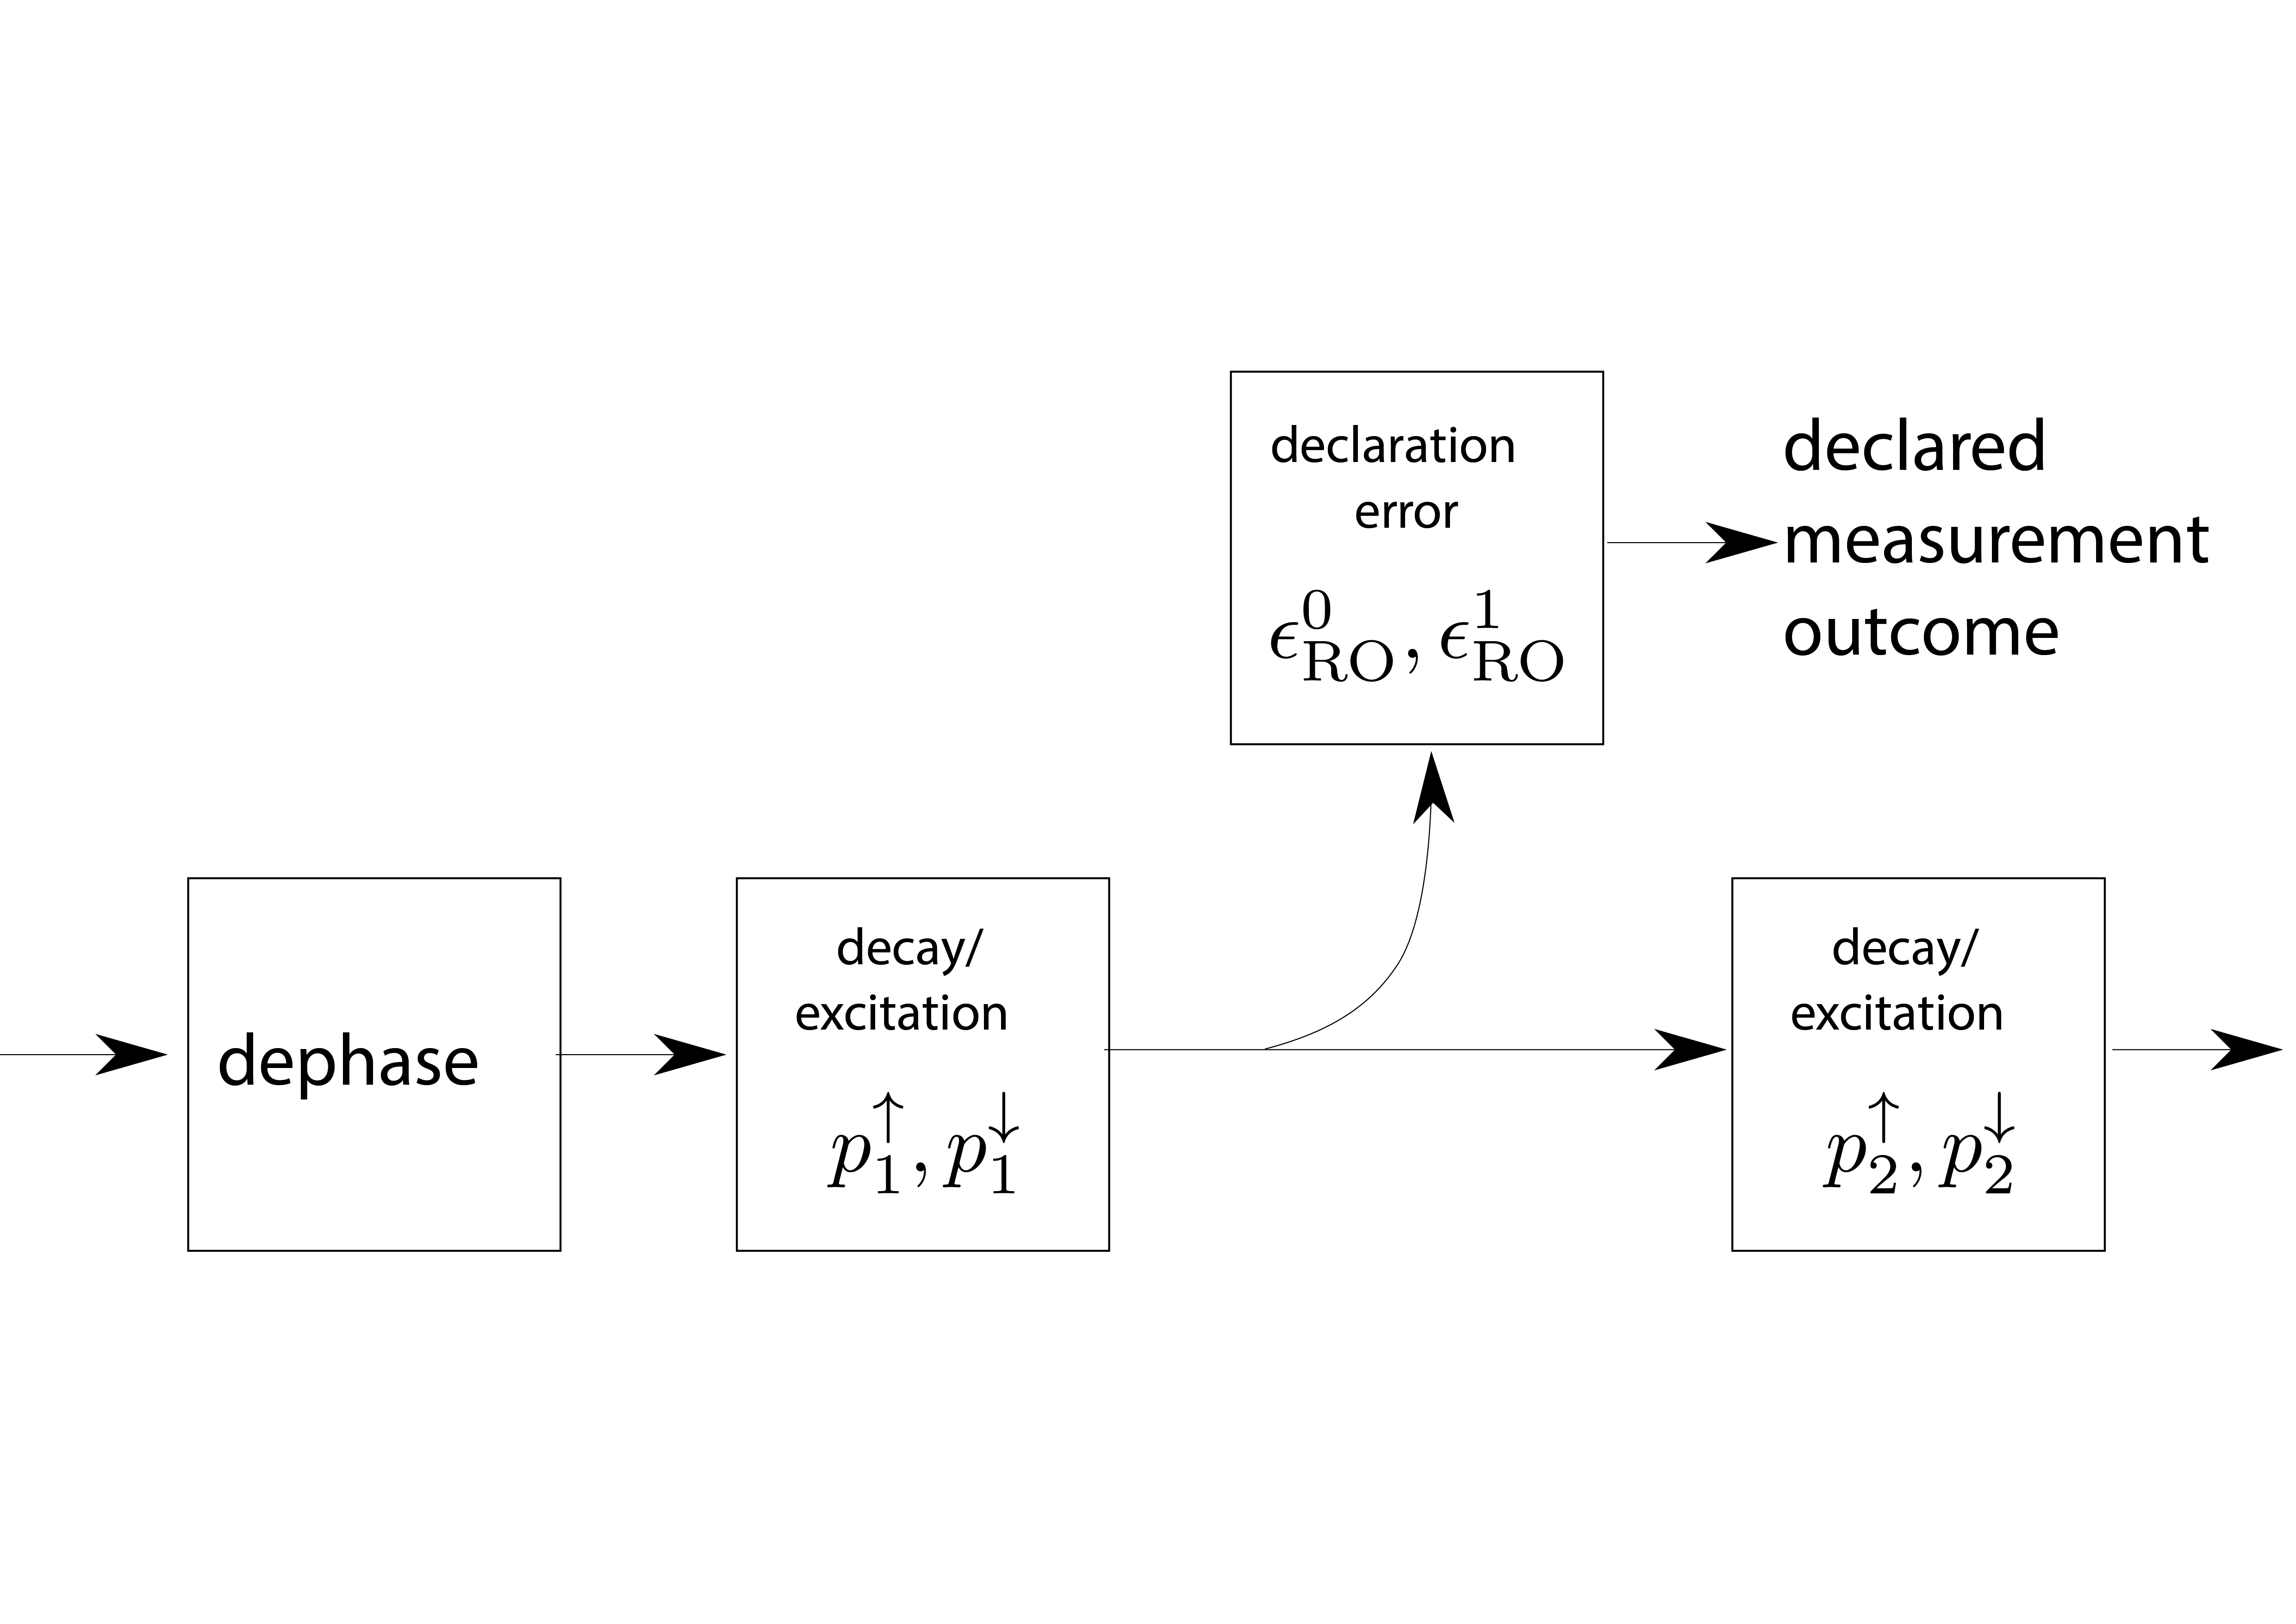
\includegraphics[width=0.5\textwidth]{figures/measure_model.png}
\caption{\label{fig:org0c4366d}
The model for measurements consists of a dephasing of the qubit followed by a period of decay and excitation with probability \(p_{\uparrow / \downarrow}^{(1)}\). At this point, the qubit state is sampled. The sampling result is subject to a declaration error \(\epsilon_{RO}\), and the qubit state is subject to further decay or excitation with probabilities \(p_{\uparrow / \downarrow}^{(2)}\) before the end of the measurement block}
\end{figure}

The initial dephasing step in the measurement model (Fig. \ref{fig:org0c4366d}) occurs due to the \hyperref[sec:org16b078d]{photon decay} effect.

"We find that the readout errors \(\epsilon_{RO}^{|i\rangle}\) are almost independent of the qubit state \(|i\rangle\), and so we describe them with a single readout error parameter \(\epsilon_{RO}\)".
The outcome-independent declaration error of \(\epsilon_{RO} = \epsilon_{RO}^{1} = \epsilon_{RO}^{0} = 0.15 \%\) is extracted from experiments. 

They ignore effects leading to measurement-induced mixing and non-linearity of the readout resonator, as well as residual photon numbers.

\item Photon decay
\label{sec:org16b078d}
In the presence of photons in a readout resonator, the coupled qubit is affected suffering a \(p_{\phi, photon}\) dephasing.
This dephasing is present whenever the coupled qubit is brought into superposition before the readout resonator has returned to the vacuum state following the last measurement.
This dephasing is then implemented via the same Pauli transfer matrix as \(R_{\Lambda_{T_{\phi}}}\).

\item Flux Noise
\label{sec:org9948b52}

During a quantum algorithm, "transmons are repeatedly moved in frequency away from their sweetspot using flux pulses, either to implement a C-Z gate or to avoid one. Away from the sweetspot, transmons become first-order sensitive to flux noise, which causes an additional random phase shift."

"As this noise typically has a \(1/f\) power spectrum, the largest contribution comes from low-frequency components that are essentially static for a single run, but fluctuating between different runs."
"Shifting the transmon from its sweetspot \(f_{q,max}\) to a lower frequency \(f_q (t)\) makes it first-order sensitive to flux noise".

"In our simulation, we approximate the effect of this noise through ensemble averaging, with quasi-static phase error added to a transmon whenever it is flux pulsed."

As one could see in the figures 4 and 5 from the Supplemental information, a little over-rotation  caused by inaccurate calibration of the flux pulse in a single- or two-qubit gate translates in a huge increase of the \(\epsilon_L\).
\end{itemize}


\item Effects not taking into account
\label{sec:org611d3b8}

They use a simple model for the CZ errors.
They neglect leakage (previous experiments have reduced leakage probability per CZ to \(\approx\) 0.3\%).
Of course this simplification is also in \textbf{quantumsim}.
\end{itemize}

\subsection*{Error Framework}
\label{sec:orgc444644}
\begin{figure}[htbp]
\centering
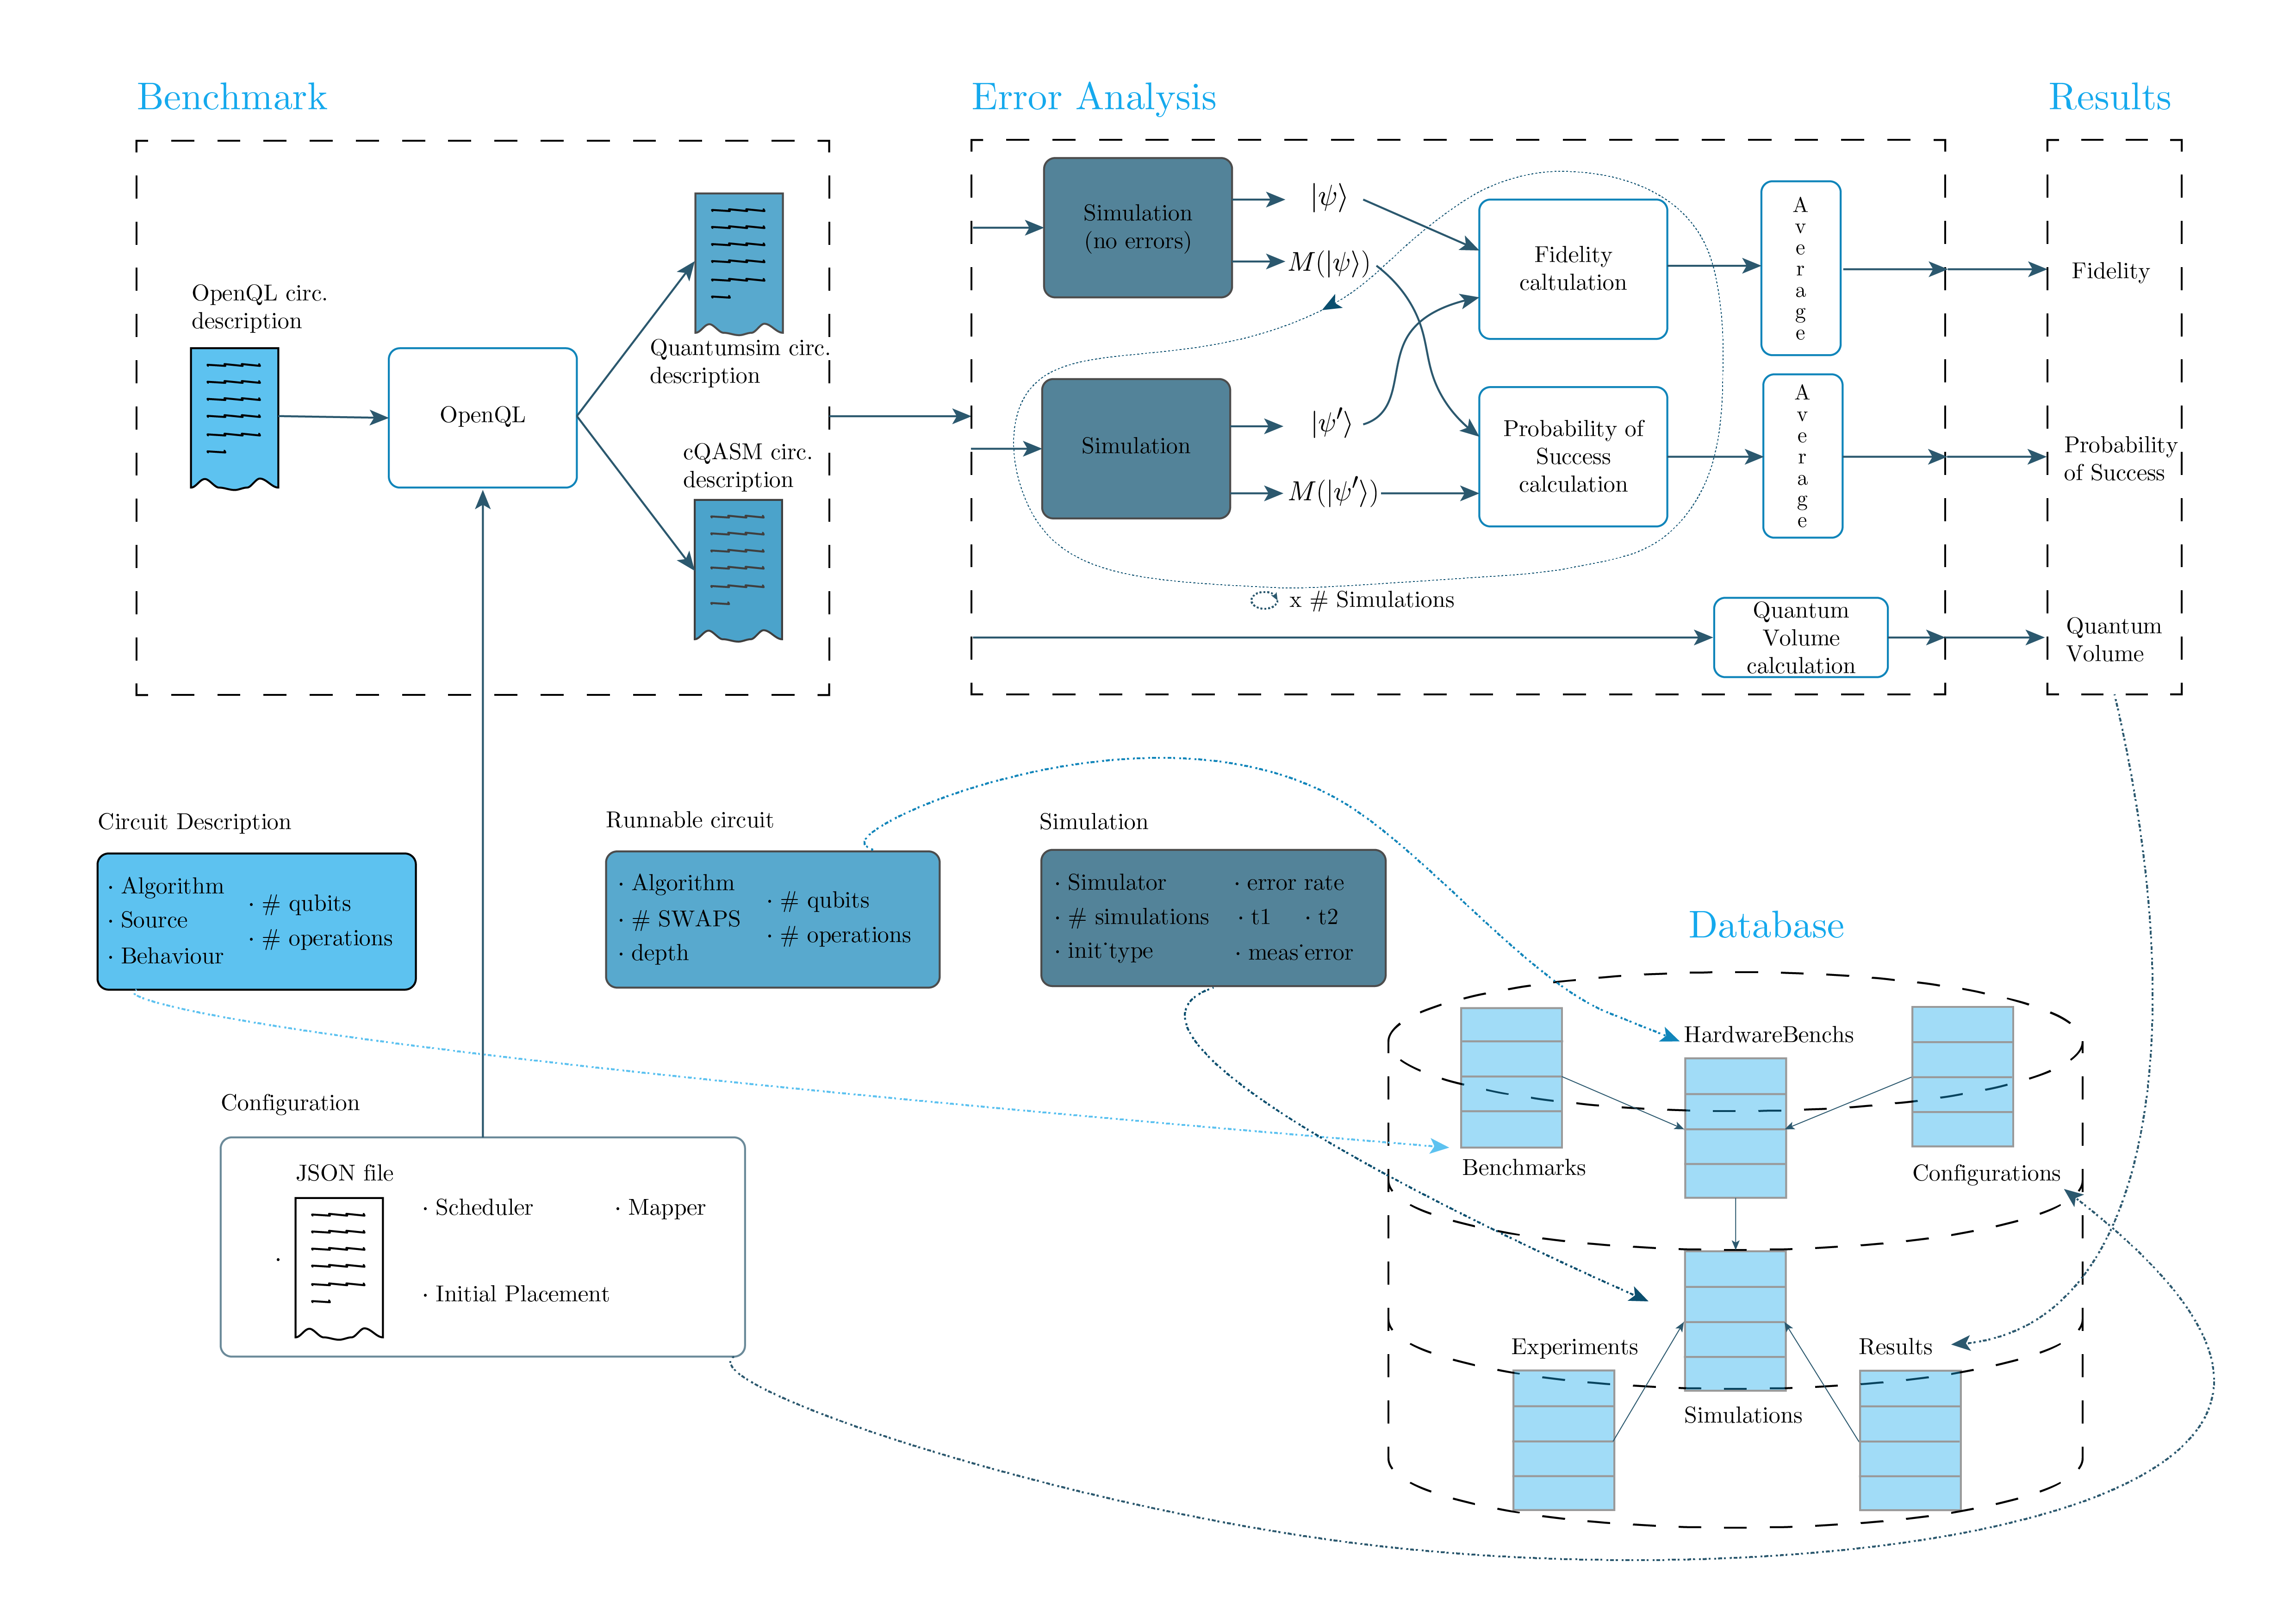
\includegraphics[width=\textwidth]{figures/error_framework_diagram.png}
\caption{\label{fig:org14e7c1e}
Error Framework}
\end{figure}

\begin{itemize}
\item Benchmark Object
\label{sec:orgc1968f3}

\begin{figure}[htbp]
\centering
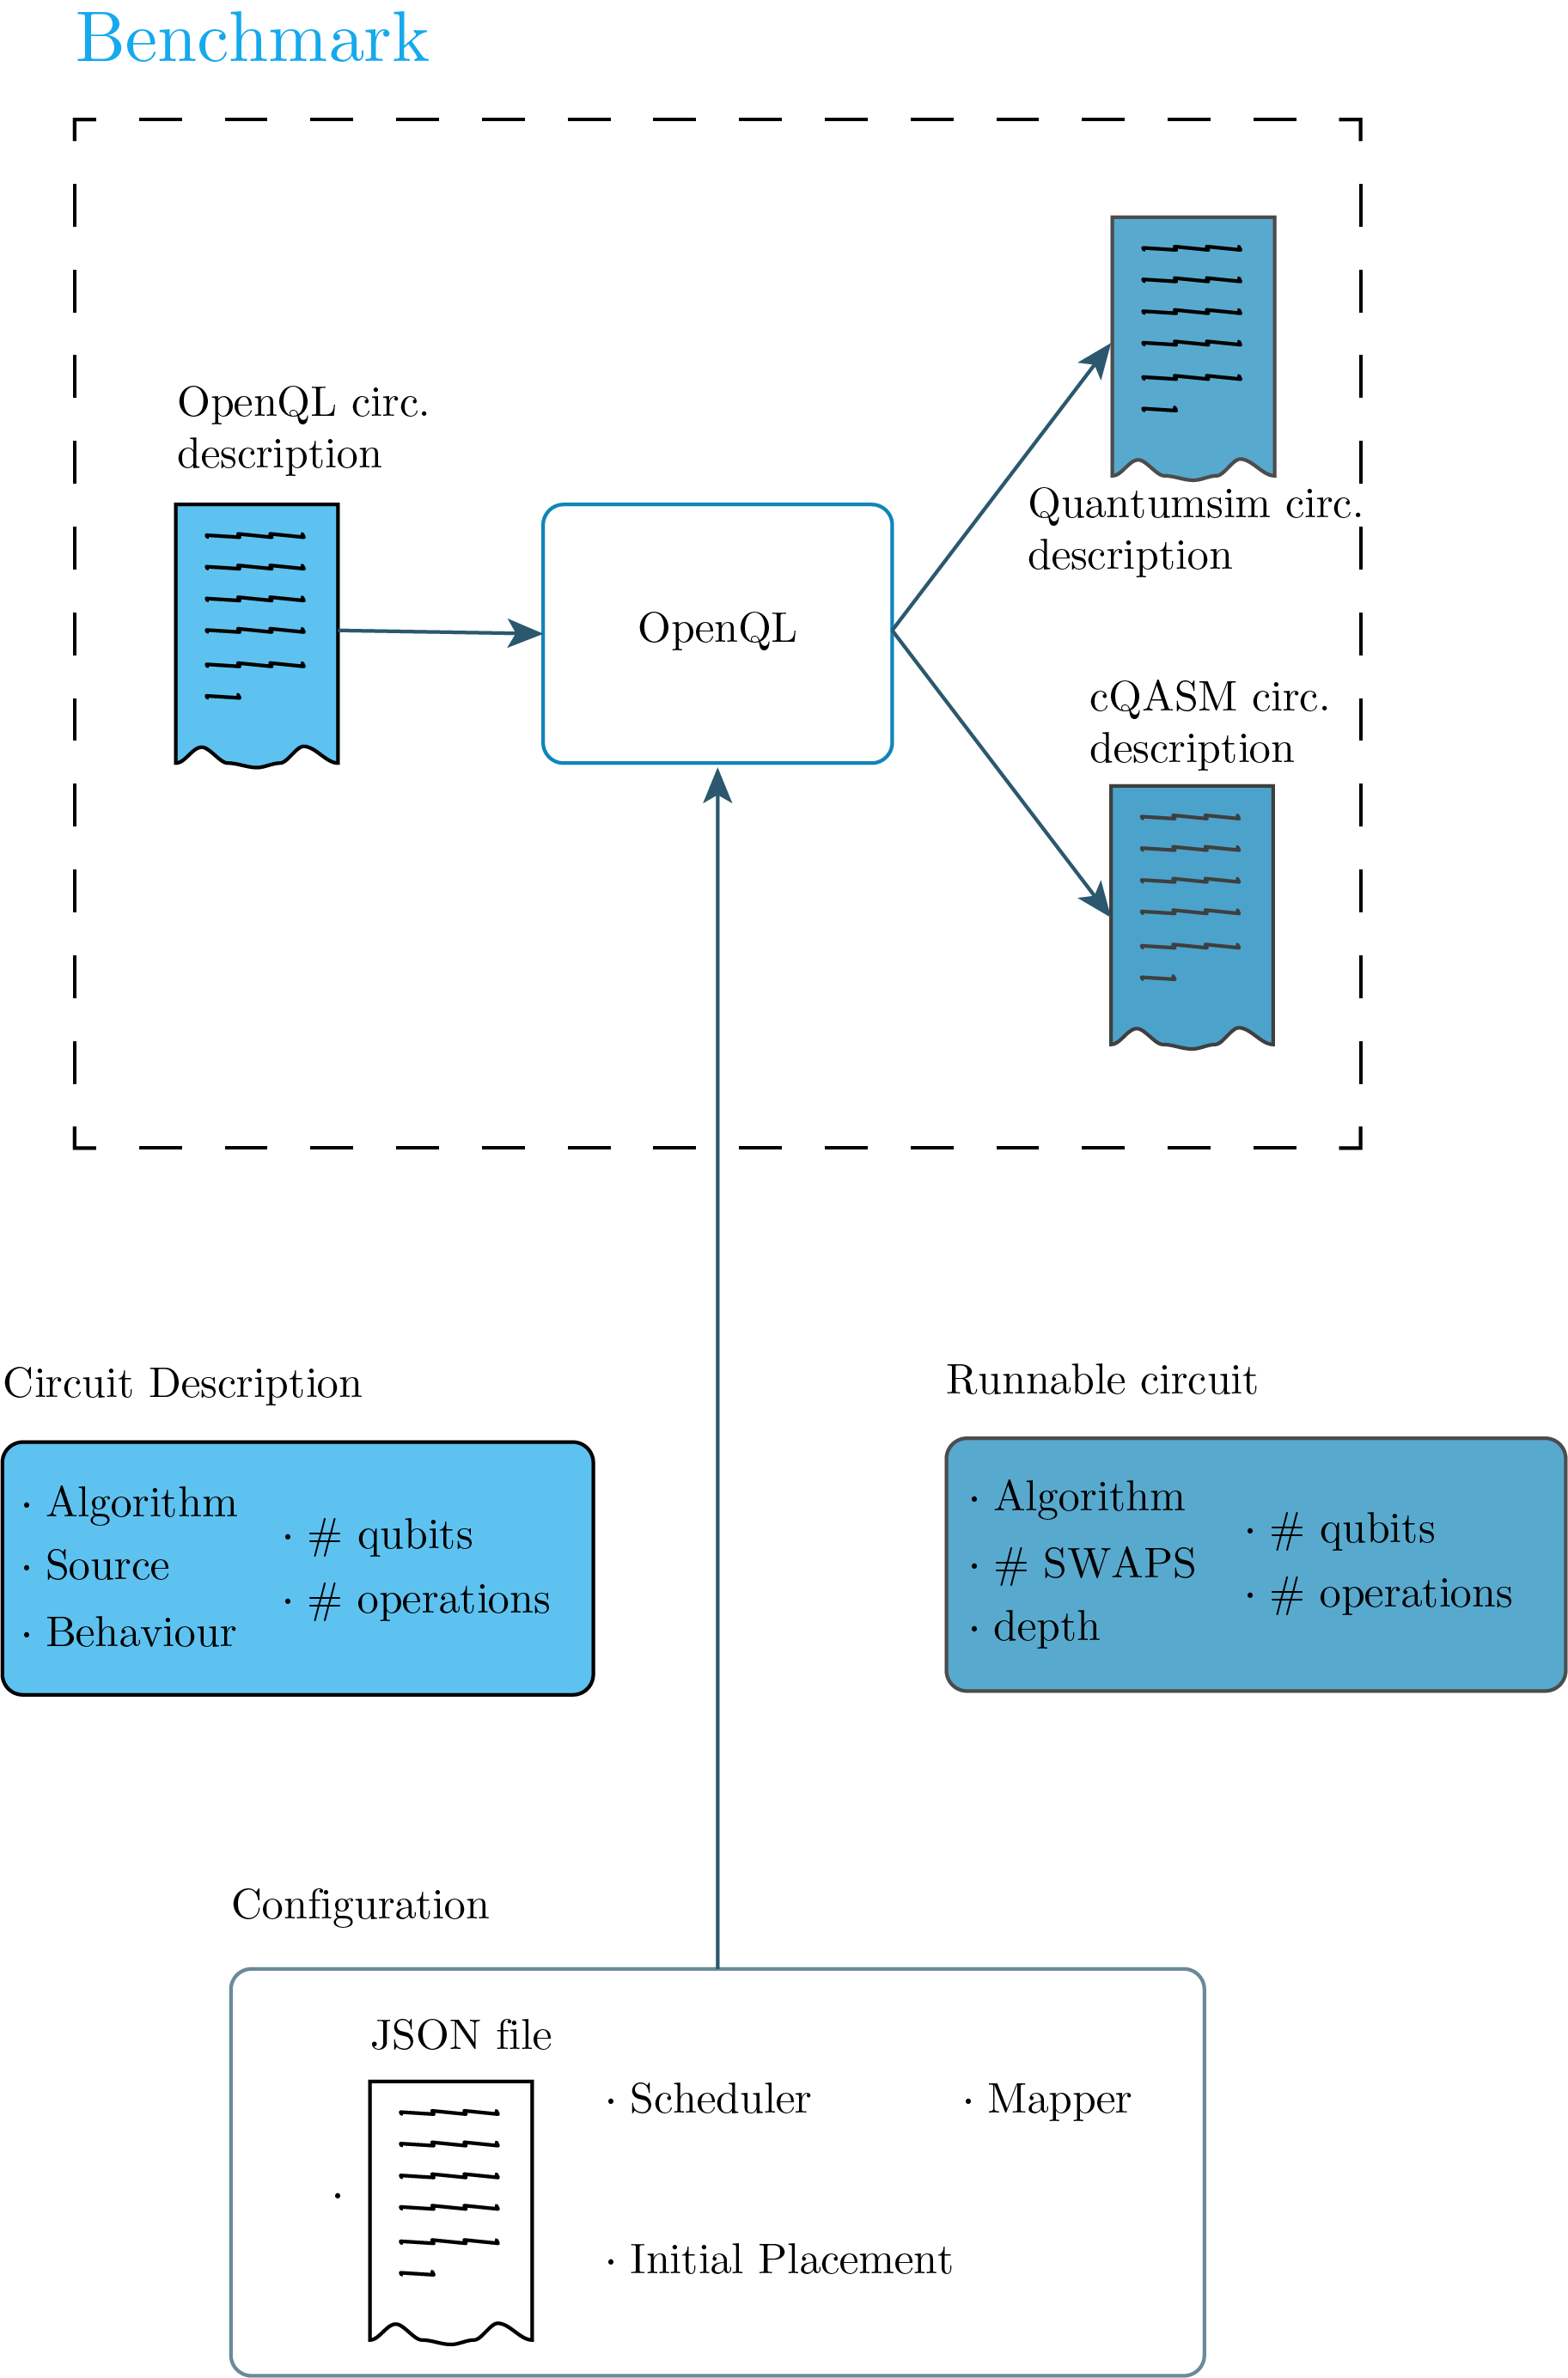
\includegraphics[width=.5\textwidth]{figures/benchmark_object.png}
\caption{\label{fig:org820b34b}
Benchmark Object \ldots{}}
\end{figure}

\item Mapping Analysis Object
\label{sec:org4a26228}

\begin{figure}[htbp]
\centering
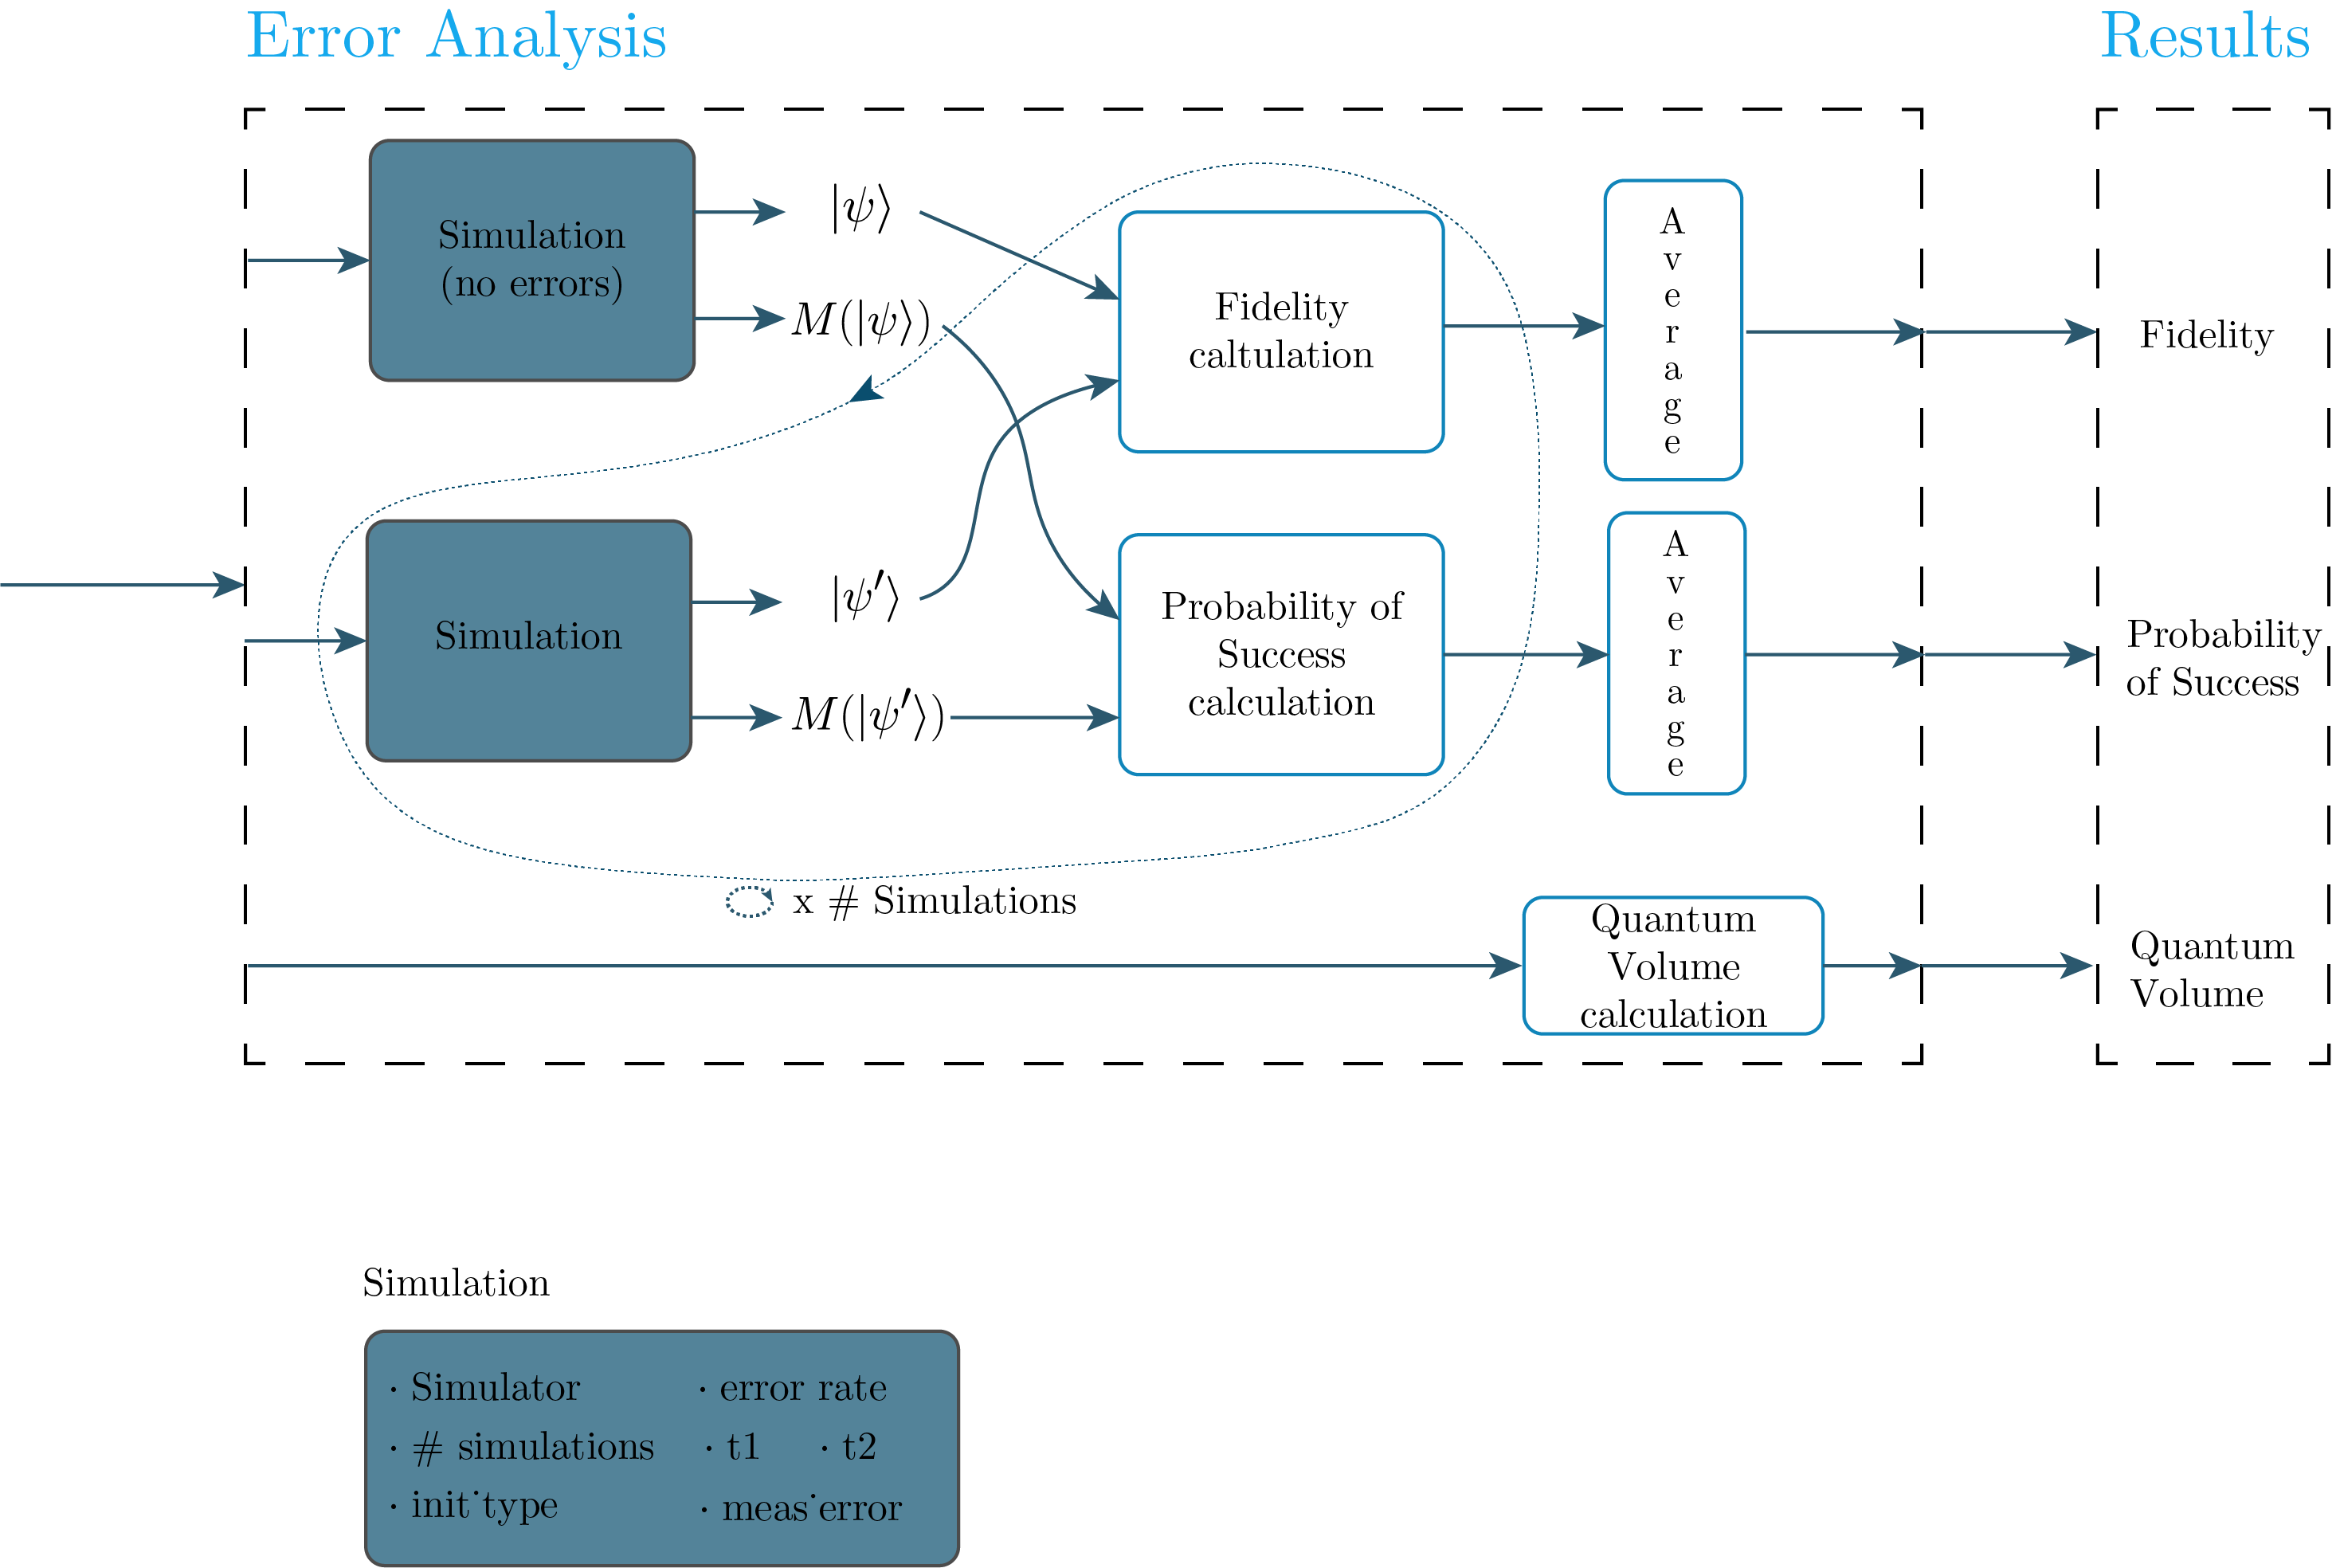
\includegraphics[width=.75\textwidth]{figures/error_analysis.png}
\caption{\label{fig:orgc987e4f}
Mapping Analysis Object \ldots{}}
\end{figure}

\item Database
\label{sec:orge4c1797}

\begin{figure}[htbp]
\centering
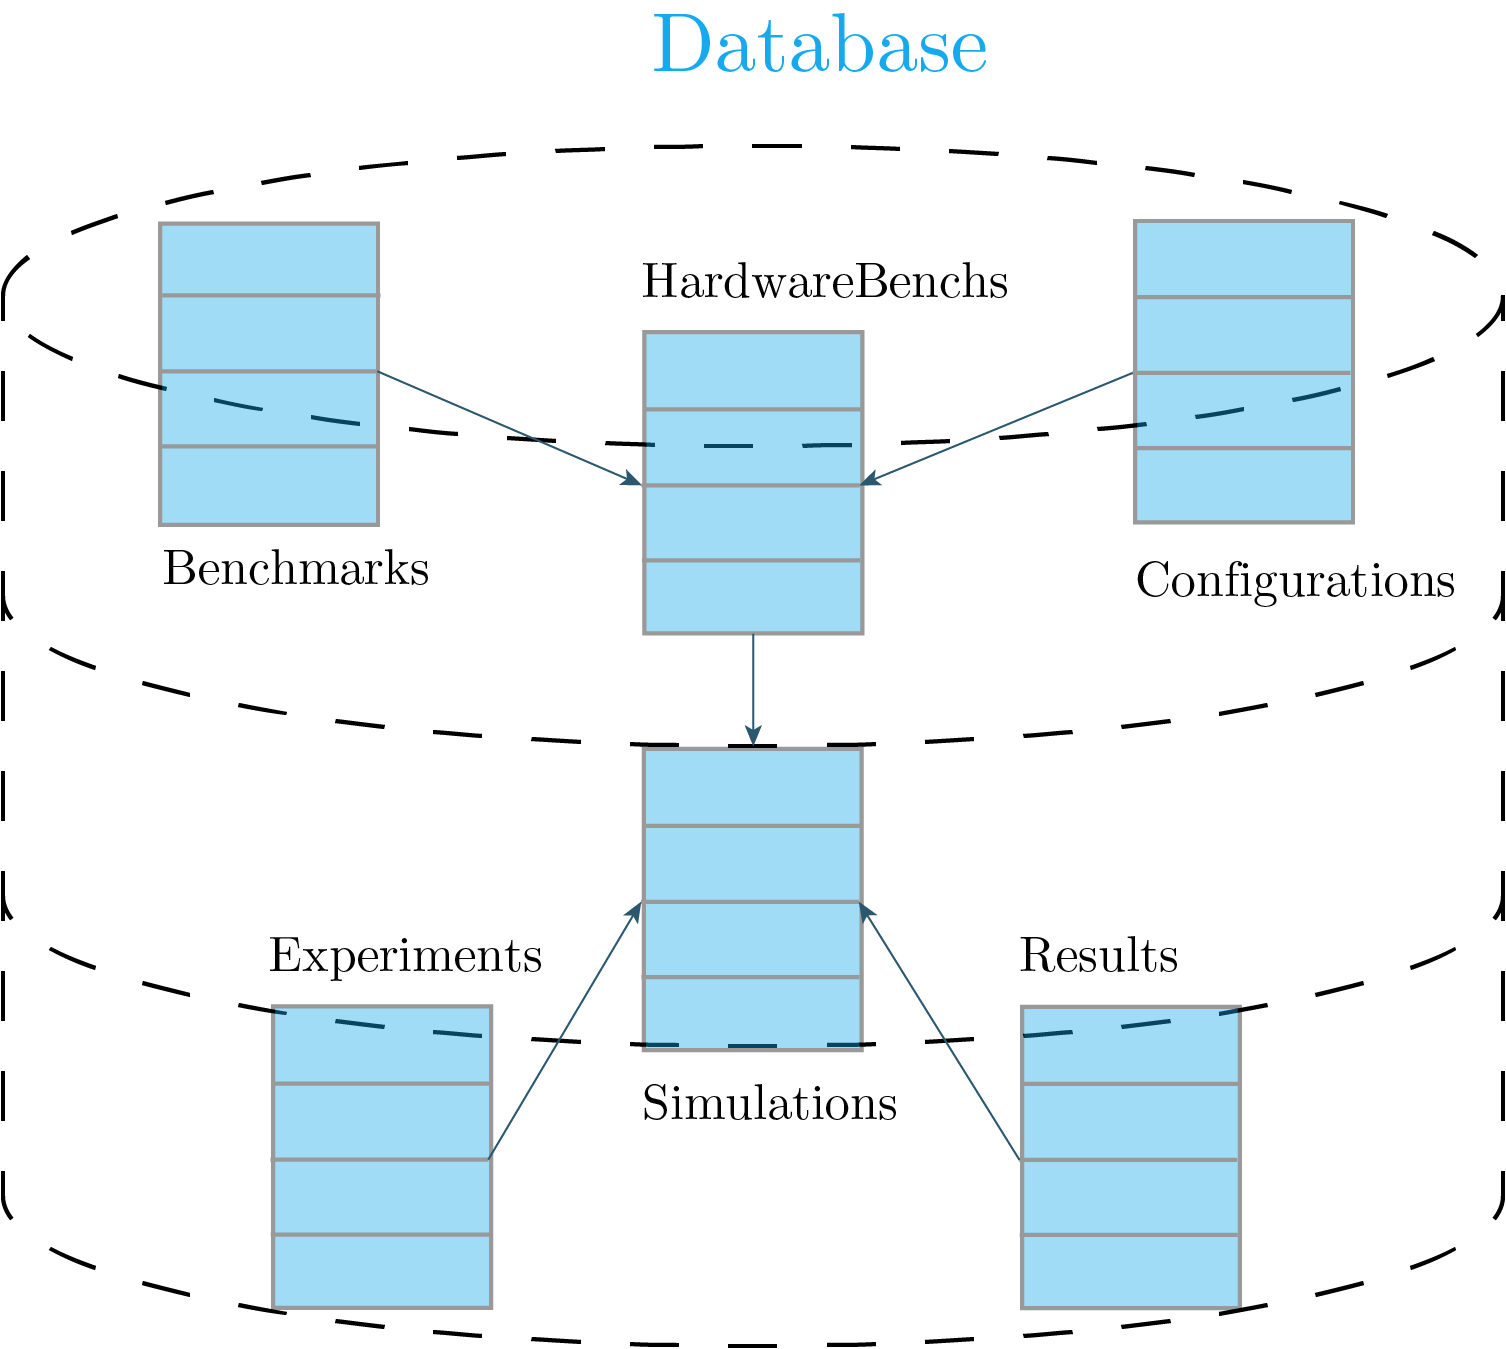
\includegraphics[width=.5\textwidth]{figures/database_scheme_detail.png}
\caption{\label{fig:orgfdf8b19}
Database tables}
\end{figure}

\begin{figure}[htbp]
\centering
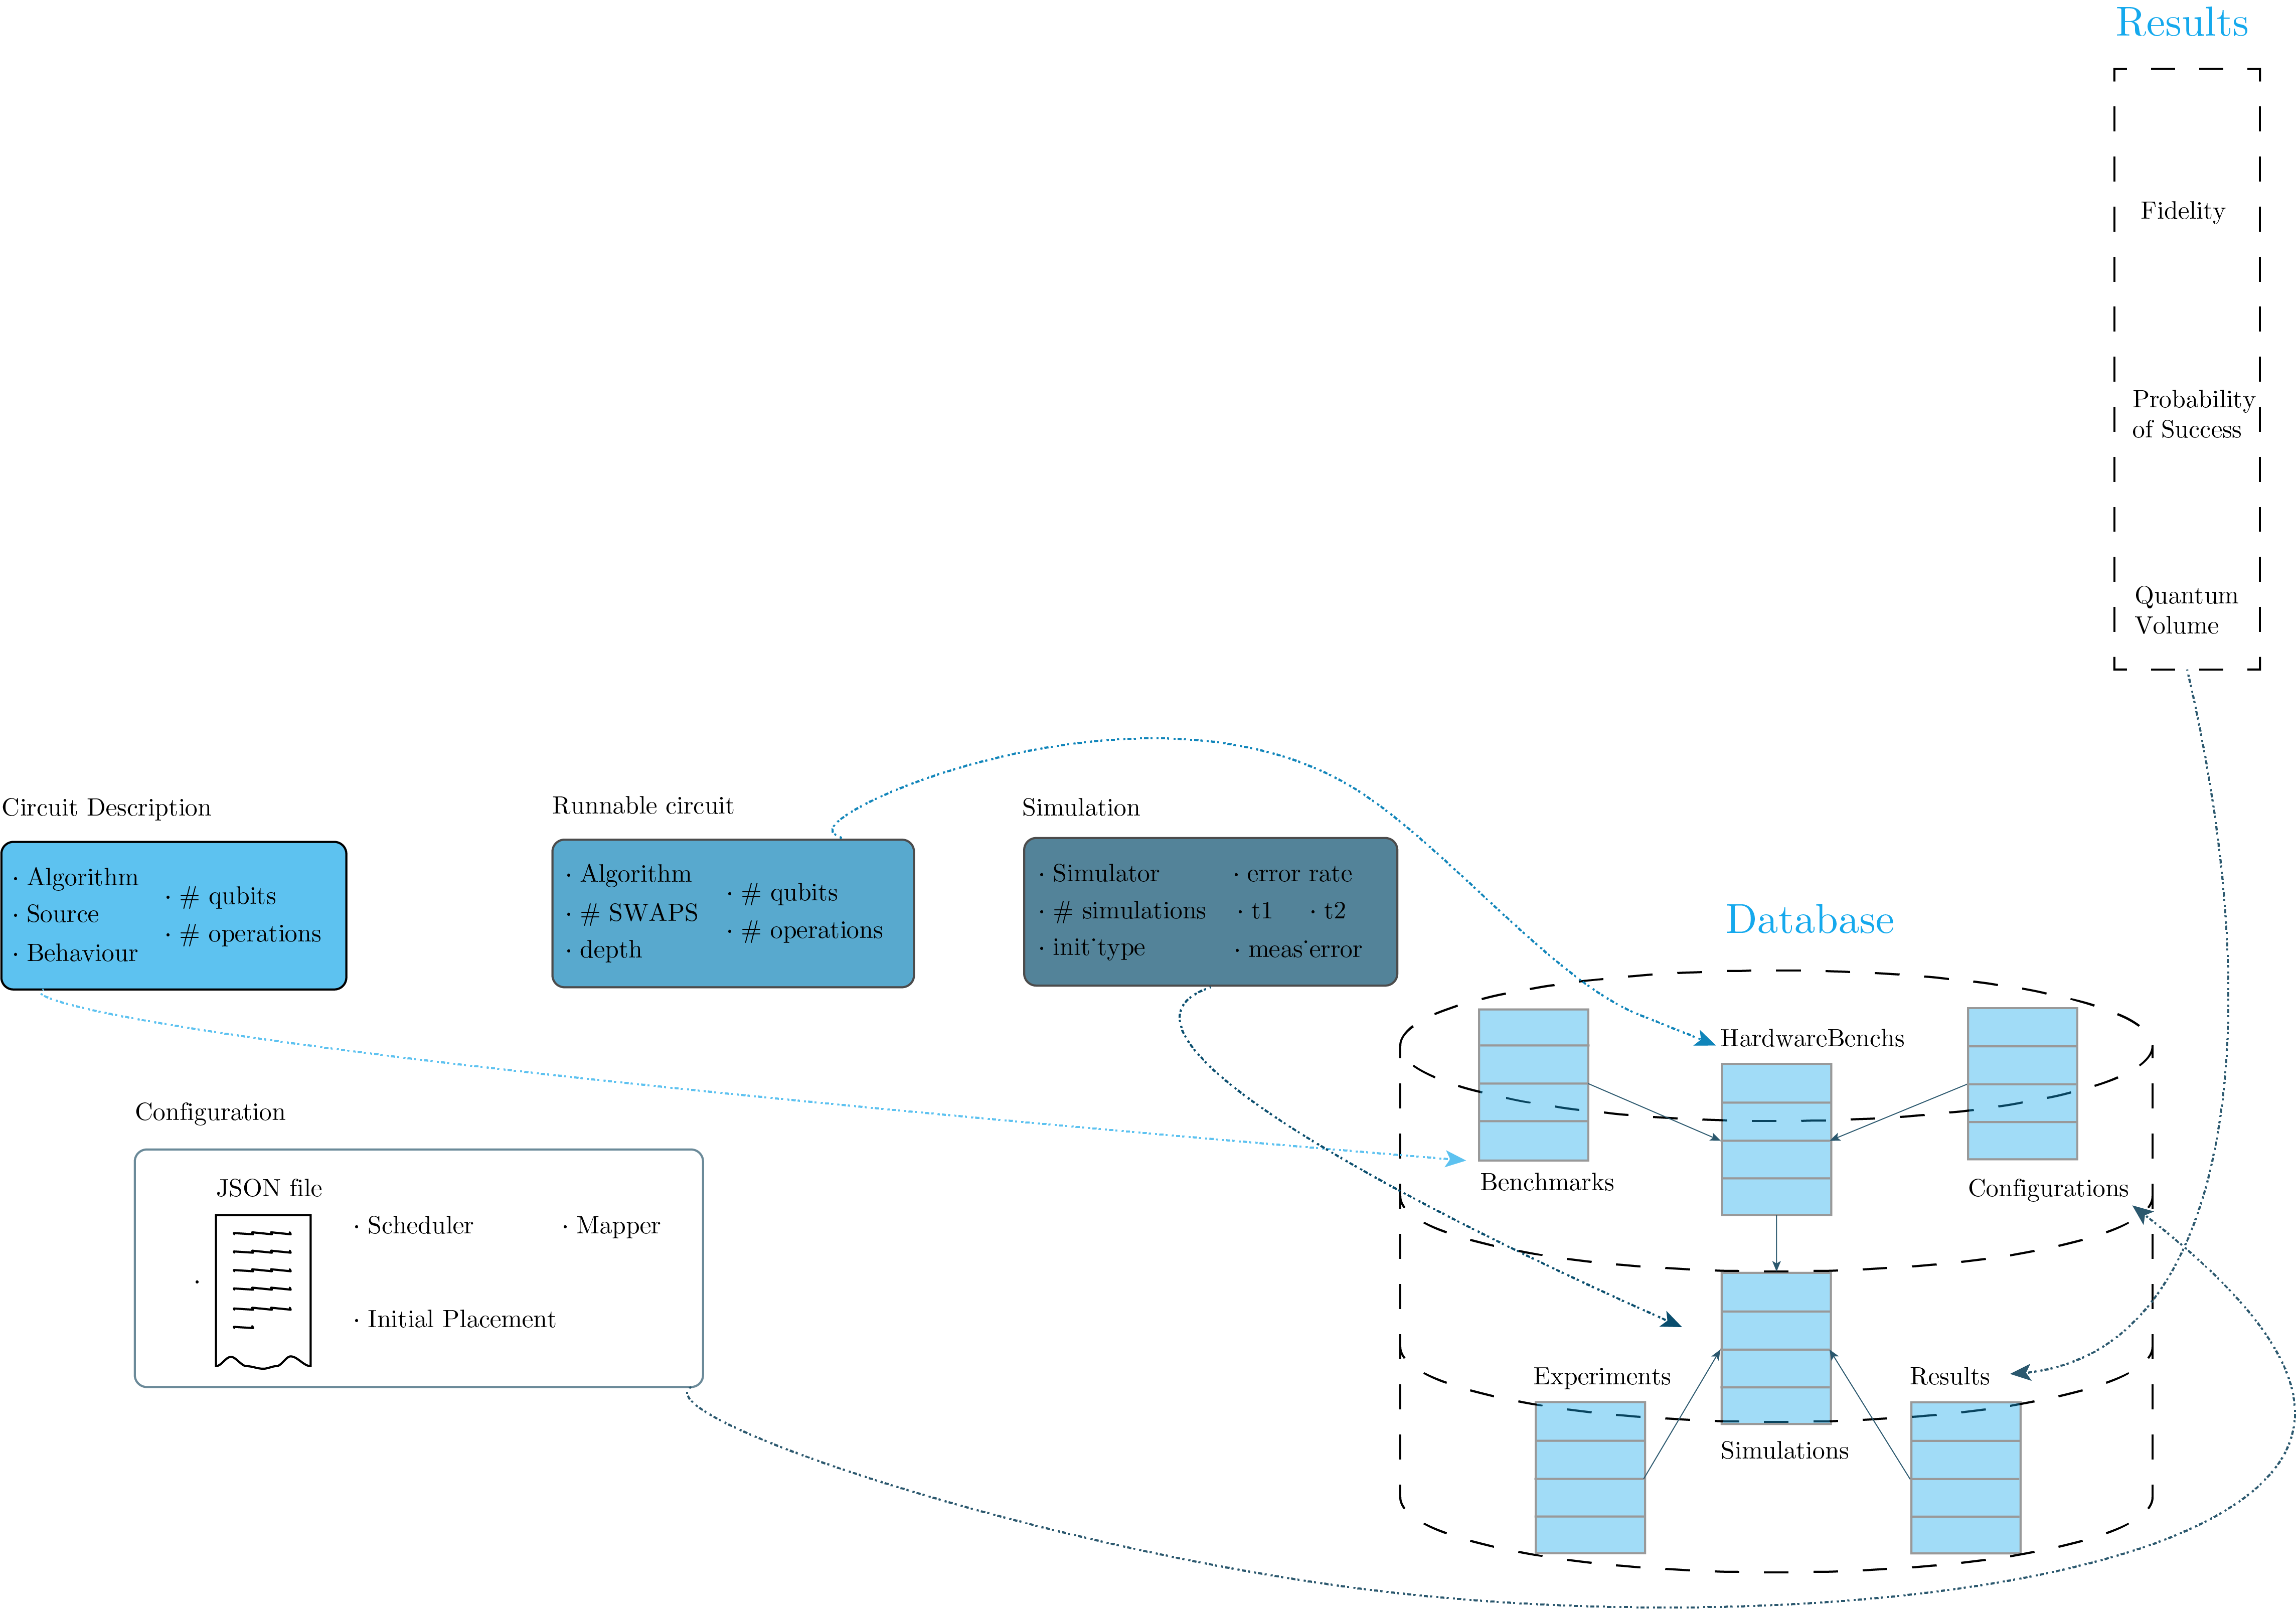
\includegraphics[width=\textwidth]{figures/database_scheme_general.png}
\caption{\label{fig:org57df4b5}
Database tables information}
\end{figure}
\end{itemize}
